\documentclass{modeleRapport}

\addbibresource{biblio.bib}

%--------------------------------------

\titre{Machine Learning Project}
\soustitre{ESILV A4 - DIA2}

\enseignant{Nédra \textsc{MELLOULI} \\
            Zachary \textsc{FAKIR} }

\eleves{Nour \textsc{AFFES} \\
	Lucas \textsc{BLANCHET} \\ 
	Hugo \textsc{BONNELL} \\
    Rayan \textsc{HAMADEH}}

%--------------------------------------

\begin{document}

\fairepagedegarde
\fairetabledesmatieres

%--------------------------------------

\section{Pre-Project}

\subsection{Problem Definition}

Drowsy driving, a serious hazard often resulting from insufficient rest, causes drivers to lose focus, react more slowly, and even experience brief micro-sleeps. This issue has devastating impacts, contributing to approximately 328,000 accidents, 109,000 injuries, and 6,400 fatalities annually (Bankrate \cite{Bankrate}). Unlike the effects of alcohol or drugs, drowsiness is harder to detect, creating a challenge for preventive measures. A 2019 AAA Foundation \cite{AAAFoundation} study reveals that while 96\% of drivers recognize the extreme risk of drowsy driving, only 29\% feel that they are at risk of getting pulled over by law enforcement. 


\subsubsection{Existing technologies}

\begin{itemize}
\item \textbf{Mercedes-Benz ATTENTION ASSIST} \cite{Mercedes}: analyzes driving pattern in the first few minutes of the ride, and then detects patterns that might be due to fatigue, and alerts by a coffee cup symbol on the dashboard.  

\item F\textbf{ord Driver Alert System} \cite{Ford}: monitor level of alertness based on driving behavior, an alert is displayed on the information display, that will be automatically cleared after a while and can also be cleared by pressing ok on the steering wheel. This feature can be turned off and will stay off even if you turn the ignition off and back on. This method can be impacted by windshield conditions such as bird droppings, ice, or snow. System is only available at speeds below activation speed (64 km/h) Proposed Solution and Business Objectives. 
\end{itemize}

Our project aims to develop a machine-learning-powered system that monitors driver fatigue in real-time. This solution will leverage a camera-based approach, ideally suited to modern vehicles already equipped with interior cameras. Unlike current technology, this model will focus directly on the driver’s condition by analyzing eye and mouth states, reducing dependence on external driving conditions. 

\subsubsection{Key business objectives}

\begin{itemize}

\item \textbf{Increase Road Safety :} By alerting drivers when drowsiness indicators are detected, the system can help prevent accidents. 

\item \textbf{Enhance Detection Accuracy :} Monitoring eye and mouth states ensures fatigue detection remains consistent across different road, traffic, and weather conditions. 

\item \textbf{Offer a Scalable Solution :} Using a straightforward dataset and CNN model, the system is designed to integrate smoothly into existing vehicle technology, avoiding significant production costs. 

\item \textbf{Foundation for Advanced Safety Features :} In future applications, the model could work with autonomous driving technology to execute actions like parking assistance or alerting emergency services if the driver fails to respond. 

\end{itemize}

\subsection{Dataset Description}

The dataset \cite{Dataset} for this project contains labeled images indicating whether a driver’s eyes are “open” or “closed” and mouth states as “yawn” or “no yawn.” This binary classification structure aligns well with a CNN model, allowing us to detect drowsiness through simple yet reliable features, focusing on real-time driver monitoring. By building a robust CNN on this well-labeled dataset, we emphasize a driver-centric approach, which addresses existing technology gaps in driver fatigue detection. 

\subsection{Scope}

The scope of this project covers the development, testing, and evaluation of a computer vision-based drowsiness detection model. Key components include: 

\begin{itemize}

\item \textbf{Model Development :} Implementing a Convolutional Neural Network (CNN) to accurately classify eye and mouth states from real-time image data. These classifications will enable reliable identification of closed eyes or yawning—critical indicators of drowsiness. 

\item \textbf{Real-Time Deployment Potential :} Optimizing the model architecture to minimize latency, with potential for integration into embedded vehicle systems. 

\item \textbf{Driver-Centric Focus :} The model will monitor the driver’s physical state, making it adaptable to various driving environments, road types, and vehicle models. 

\item \textbf{Alert System :} Although primary development focuses on detection accuracy, we will outline alert system recommendations to ensure the notifications are clear and hard to ignore for drowsy drivers. 

\end{itemize}

\subsection{Organization}

A structured Gantt chart outlines each phase of this project, helping to ensure timely and organized progression. The tasks are divided into four major phases: Implementing a standard solution, improving it for stage 2, further improvements for stage 3 and finally, Report and Presentation Preparation. Each task is designed with inter-dependencies in mind, ensuring a streamlined workflow and timely completion of project milestones.

%---------------------------------------

\section{Stage 1}

\subsection{Problem Formalization}
\subsubsection{Problem Statement}
The primary objective here is to develop a machine-learning-powered system that monitors driver fatigue in real-time. This model will focus directly on the driver’s condition by analyzing eye and mouth states and deduce if the driver is in a tired state accurately.
\subsubsection{Understanding the Dataset}
As we said before, our dataset consists of labeled images indicating whether a driver’s eyes are “open” or “closed” and mouth states as “yawn” or “no yawn.” The data is balanced: we have the same distribution between classes (726 for both closed and open and 723/725 for yawn and no yawn respectively) so we won’t have an issue with biased model prediction or poor performance on minority class. \\

\textbf{Dataset Overview:} \\
\begin{table}[H]
    \centering
    \begin{tabular}{|c|c|c|c|}
        \hline
        Eye Closed & Eye Opened & Mouth Yawn & Mouth no Yawn \\
        \hline
        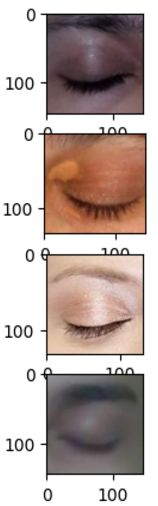
\includegraphics[width=3cm]{Images/eyeClosed.png}
        &
        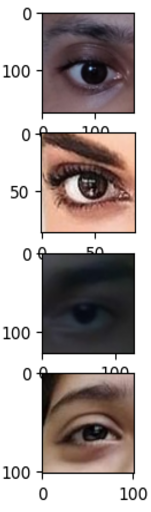
\includegraphics[width=3cm]{Images/eyeOpen.png}
        &
        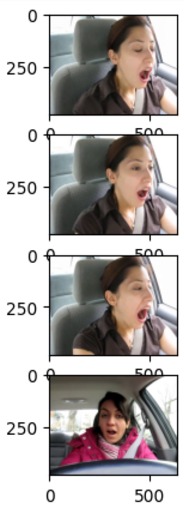
\includegraphics[width=3cm]{Images/yawn.png}
        &
        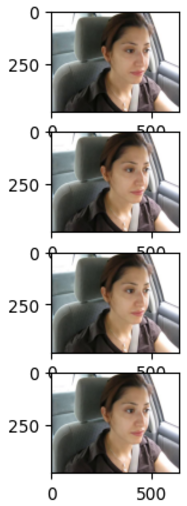
\includegraphics[width=3cm]{Images/noYawn.png}
        \\
        \hline
    \end{tabular}
    \caption{Un tableau simple.}
\end{table}

We notice that the images don't share the same format, we'll thus be tackling this issue.

\subsection{Refining the Dataset}
Our initial task involved meticulously cleaning and pre-processing the data. This process was crucial to ensure the integrity and usability of the dataset for machine learning models. Key steps included: 
\begin{itemize}
    \item To handle missing or corrupted values.
    \item To remove duplicates if any.
    \item To make sure that all pictures have the same size. 
\end{itemize}

\subsection{Evaluation Metrics}

In addition to \textbf{accuracy}, we considered other metrics like \textbf{precision, recall, and F1 score} for a comprehensive assessment of our models. These metrics provided a more nuanced view of the model's performance because we need to be as accurate as possible. 

\subsection{Data cleaning and pre-processing}

In the process of preparing our data for our machine learning project, our group followed a set of essential steps.

\begin{codebox}[Data cleaning]{Checking for missing or corrupted data \texttt{Python}}
\begin{minted}{python}
from PIL import Image
import os

def count_corrupted_images(dataset_path):
    corrupted_count = 0
    total_images = 0

    for root, _, files in os.walk(dataset_path):
        for file in files:
            file_path = os.path.join(root, file)
            total_images += 1
            try:
                with Image.open(file_path) as img:
                    img.verify()
            except Exception as e:
                corrupted_count += 1
                print(f"Corrupted: {file_path} - Error: {e}")

    print(f"\nTotal Images Checked: {total_images}")
    print(f"Total Corrupted Images: {corrupted_count}")
    return corrupted_count

count_corrupted_images(path+"/train/Closed")
count_corrupted_images(path+"/train/Open")
count_corrupted_images(path+"/train/yawn")
count_corrupted_images(path+"/train/no_yawn")
\end{minted}
\end{codebox}

\begin{codebox}[OutputA]{ Output of Code 1}
Total Images Checked: 726\\
Total Corrupted Images: 0\\
\\
Total Images Checked: 726\\
Total Corrupted Images: 0\\
\\
Total Images Checked: 723\\
Total Corrupted Images: 0\\
\\
Total Images Checked: 725\\
Total Corrupted Images: 0\\
\end{codebox}

We don't have any corrputed file in the dataset. Let's check for duplicates:

\begin{codebox}[Duplicate Check]{Checking for duplicate data \texttt{Python}}
\begin{minted}{python}
import hashlib
import cv2
import os

def remove_duplicates(dataset_path):
    image_hashes = {}
    unique_images = []

    for root, _, files in os.walk(dataset_path):  
        for file in files:
            file_path = os.path.join(root, file)  

            img = cv2.imread(file_path, cv2.IMREAD_GRAYSCALE)

            img_bytes = img.tobytes()

            img_hash = hashlib.md5(img_bytes).hexdigest()

            if img_hash not in image_hashes:
                image_hashes[img_hash] = file_path
                unique_images.append(file_path)
            else:
                return(f"Duplicate found: {file_path}")

    return ("There are no duplicate images")

# Example usage:
# Assuming 'path' is your base dataset path
remove_duplicates(path + "/train/Closed")
remove_duplicates(path + "/train/Open")
remove_duplicates(path + "/train/yawn")
remove_duplicates(path + "/train/no_yawn")
\end{minted}
\end{codebox}

\begin{codebox}[OutputB]{ Output of Code 3}
'There are no duplicate images'
\end{codebox}

As stated, the pictures are all unique, we can use all of them.

Finally, we will use some pre-processing techniques such as:\\
\begin{itemize}

\item \textbf{Image Transformation} to make all the image have the same size and increases the accuracy.\\

\begin{codebox}[Image Transformation]{Image transformation - resize images \texttt{Python}}
\begin{minted}{python}
def load_images(dataset_path, target_size=(64, 64)):
    images = []
    labels = []
    for label in os.listdir(dataset_path):
        class_path = os.path.join(dataset_path, label)
        if not os.path.isdir(class_path):
            continue
        for img_file in os.listdir(class_path):
            img_path = os.path.join(class_path, img_file)
            img = cv2.imread(img_path, cv2.IMREAD_GRAYSCALE) 
            if img is not None:
                img_resized = cv2.resize(img, target_size) 
                images.append(img_resized.flatten())
                labels.append(label)
    return np.array(images), np.array(labels)

images, labels = load_images(path+'/train')
\end{minted}
\end{codebox}

\item \textbf{Normalization} to creates a consistency in pixel value ranges for better training and numerical stability, to make every pixel of the image having a value between 0 and 1 instead of 0 and 255.\\

\begin{codebox}[Image Normalization]{Normalize images \texttt{Python}}
\begin{minted}{python}
X, y = load_images(path+'/train')
X = X/255.0
\end{minted}
\end{codebox}

\end{itemize}

/insererbiblio
\end{document}
